\chapter{\texttt{piped}}

In the previous chapter, I described the Master-Worker paradigm conceptually. In this chapter, we look at one specific piece of software that implements this concept. The software is called `piped'. piped\index{Linux commands!piped@\texttt{piped}} is a so-called \textit{daemon}\index{daemon}, i.e.\,a program that does not have an graphical interface but instead runs in the background\footnote{\burl{http://en.wikipedia.org/wiki/Daemon\_\%28computing\%29}}. Its task is to manage the communication between the master node and the workers (see Fig.~\ref{fig:piped}). The Master now only has to tell piped which tasks it wants to evaluate, and wait for the results while the piped program takes care of the logistics of communicating with the Worker nodes.

You can check if \lstinline[style=bashinline]{piped} is already running by checking the processes that are running system-wide:
\begin{lstlisting}[style=basic,style=bash] 
jspaaks@login4:~$ ps -ef
\end{lstlisting}
and then filter the long list of results with the \lstinline[style=bashinline]{grep} program:
\begin{lstlisting}[style=basic,style=bash]
jspaaks@login4:~$ ps -ef|grep ruby
jspaaks  17312 17193  0 00:14 pts/5    00:00:00 ruby1.9.1 ./piped.rb
jspaaks  17363 17193  0 00:14 pts/5    00:00:00 grep ruby
jspaaks@login4:~$ 
\end{lstlisting}\index{Linux commands!ps@\texttt{ps}}\index{Linux commands!grep@\texttt{grep}}

If there is an old \lstinline[style=bashinline]{piped} still running, you must terminate it using the \lstinline[style=bashinline]{kill} command followed by the identifier of the process, e.g.
\begin{lstlisting}[style=basic,style=bash]
jspaaks@login4:~$ kill 17312
\end{lstlisting}\index{Linux commands!kill@\texttt{kill}}
otherwise the messages from different \lstinline[style=bashinline]{piped} instances will get intermixed.

\begin{figure}[htb]
  \centering
    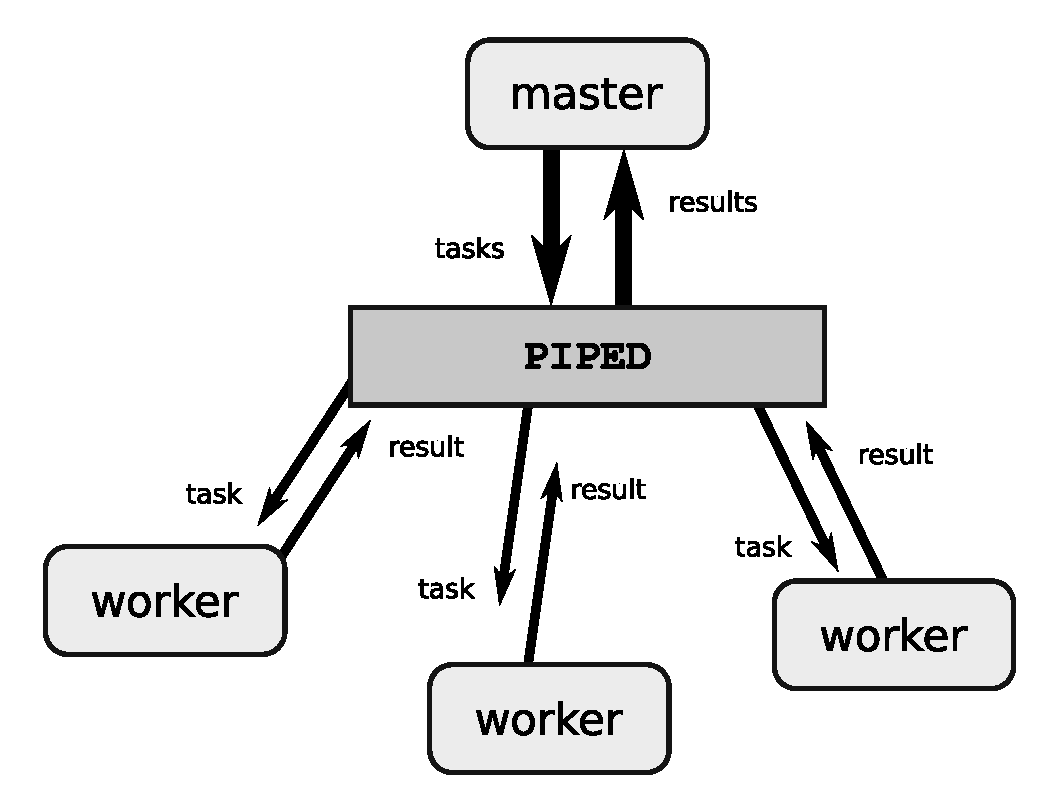
\includegraphics[width=0.9\textwidth]{./../eps/piped.eps}
  \caption{Message passing between a master node and its workers.}
  \label{fig:piped}
\end{figure}



Besides piped, there are various other softwares that implement the Master-Worker paradigm. The most commonly used Master-Worker software is probably MPI\index{Message Passing Interface}\index{MPI}, which stands for \textit{Message Passing Interface}. 
